\section{Numerical examples}
\label{sec:num-examples}
In this section, we present a numerical example to demonstrate the capability of the proposed model. To verify the implementation, we performed several other numerical experiments in \ref{Sec:App}.

In this example, we investigate the fracture propagation in a square plate with a pressurized CO$_2$ flow, with \cite{ishida2016features, wang2018influence} as the benchmarks. The specimen has edge lengths of $L=170$ mm. The geometric setup and boundary conditions are depicted in Figure \ref{Fig:Gas_geometry}. The sample is discretized into 4,832 three-noded triangular elements so that the mesh size $h\approx 5.68$ mm is obtained. Also, we set $\ell=1.6$ mm. Table \ref{Tab:Gas_input} shows the remaining parameters to be input.

\begin{figure}[htbp]
	\centering
	\includegraphics[width=0.8\textwidth]{GasFrackingModel2}
	\caption{Schematic of a cracked square plate (unit: mm) with pressurized CO$_2$ flow.}
	\label{Fig:Gas_geometry}
\end{figure}

As in Figure \ref{Fig:Gas_geometry}, there exist two preexisting fractures representing the perforations. We set $d=1$ for both fractures and set the Dirichlet boundary condition $d=0$ on the external boundary. The fluid is continuously injected into the central borehole with diameter $2r_0=20$ mm, until after the fractures propagate. Note that in this problem, the isothermal condition is adopted so that CO$_2$ is in the supercritical phase ($T=45^{\circ}$C).
%\todo[inline]{We have to mention our computation domain would be $\Omega-$ the borehole. It  is worth to mention the boundary of borehole is denoted by $\gamma_B$\\Vahid: Now that we have added Figure \ref{Fig:compute_domain}, there is no need for further explanations here.}


For the sake of simplicity, the \emph{in situ} stress is imposed on the boundary by means of its ``equivalent'' prescribed displacement. More precisely, the displacement of the same specimen with no crack under the same \emph{in situ} stress is first computed, then used as the Dirichlet boundary condition for the problem at hand. On the external boundary, we set $p=p_D$ where $p_D=0$. Moreover, $\Gamma_P=\Gamma_D$ in this example.

%\todo[inline]{YS: What is the purpose of putting a reference \cite{wang2018influence} ALONE in the title of Table \ref{Tab:Gas_input}? More words are needed, like ``according to.''\\Vahid: Changed.}

\begin{table}[htbp]
    \centering
    \caption{Default parameter values for the example. These values are taken from \cite{wang2018influence} except $g_c$, which is from \eqref{Eq:choice_ell}.}

    \begin{tabular}{l c c c}
    \hline 
         Parameters & symbol & unit& value \\
    \hline 
         Young's modulus & $E$ &MPa&  6 $\times 10^{3}$\\
         Poisson's ratio & $\nu$ &$-$&  0.34\\
         Critical energy release rate & $g_c$ &MPa$\cdot$mm&  0.306\\
         %Regularization length scale & $\ell$ &$-$&  1.6$\times 10^{-4}$\\
         Biot coefficient & $\alpha$ &$-$&  0.85\\
         Porosity & $\phi$ &$-$&  0.01\\
         Initial permeability & $k_0$ &mm$^2$&  1$\times 10^{-12}$\\
         Dynamic viscosity of  {CO}$_2$ & $\mu$ & MPa$\cdot$s& 4.04$\times 10^{-11}$\\
         %Bulk modulus of fluid & $k_f$ &$KN/mm^2$&  0.625$ \times 10^{3}$\\
        % Bulk modulus of rock & $k_s$ &$KN/mm^2$&  10$ \times 10^{3}$\\
         Initial pressure & $p_0$ &MPa&  0.1\\
         Rock's tensile strength & $\sigma_T$ &MPa&  11\\
         %Maximum principal stress & $\sigma_1$ &MPa&  1\\
         %Minimum  principal stress & $\sigma_3$ &MPa&  1\\

    \hline     
    \end{tabular}
    \label{Tab:Gas_input}
\end{table}

%\begin{figure}[htbp]
%\centering %
%\subfloat[]{
\includegraphics[width=60mm]{alpha_50.eps}\label{Fig:Gas_d_i}}
%\subfloat[]{
\includegraphics[width=60mm]{pressure_50.eps}\label{Fig:Gas_p_i}}\\
%\subfloat[]{\includegraphics[width=60mm]{alpha_75.eps}\label{Fig:Gas_d_ii}}
%\subfloat[]{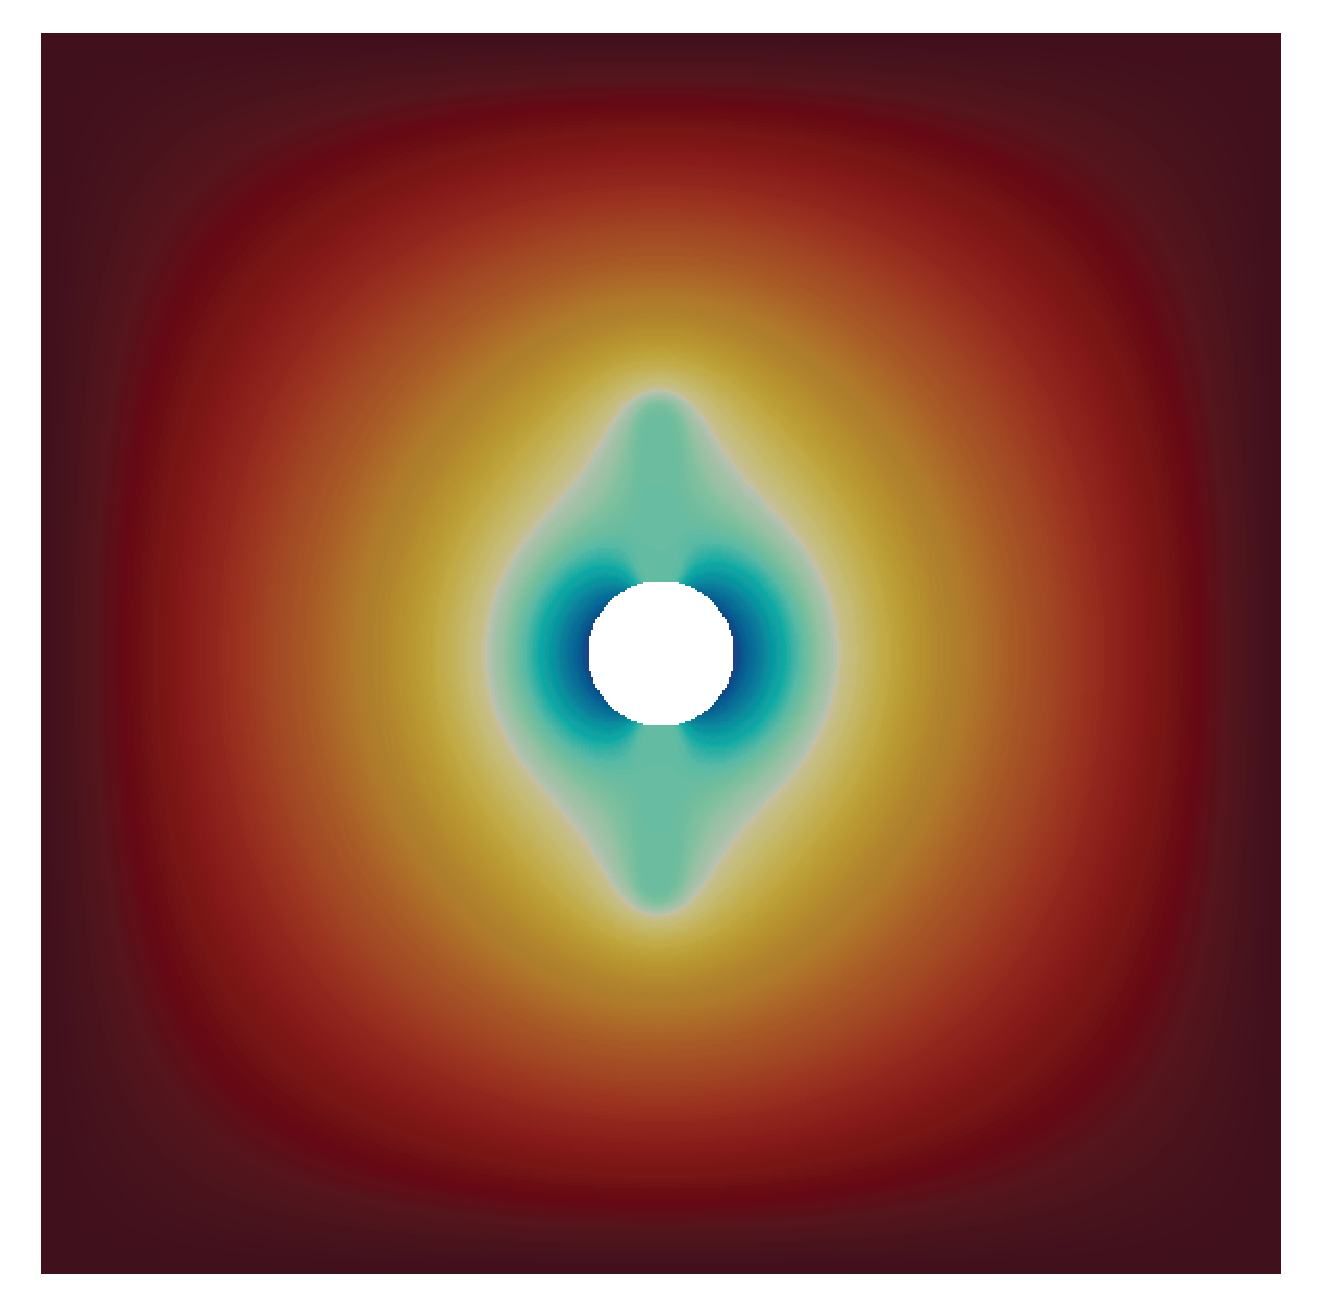
\includegraphics[width=60mm]{pressure_75.eps}\label{Fig:Gas_p_ii}}\\
%\subfloat[]{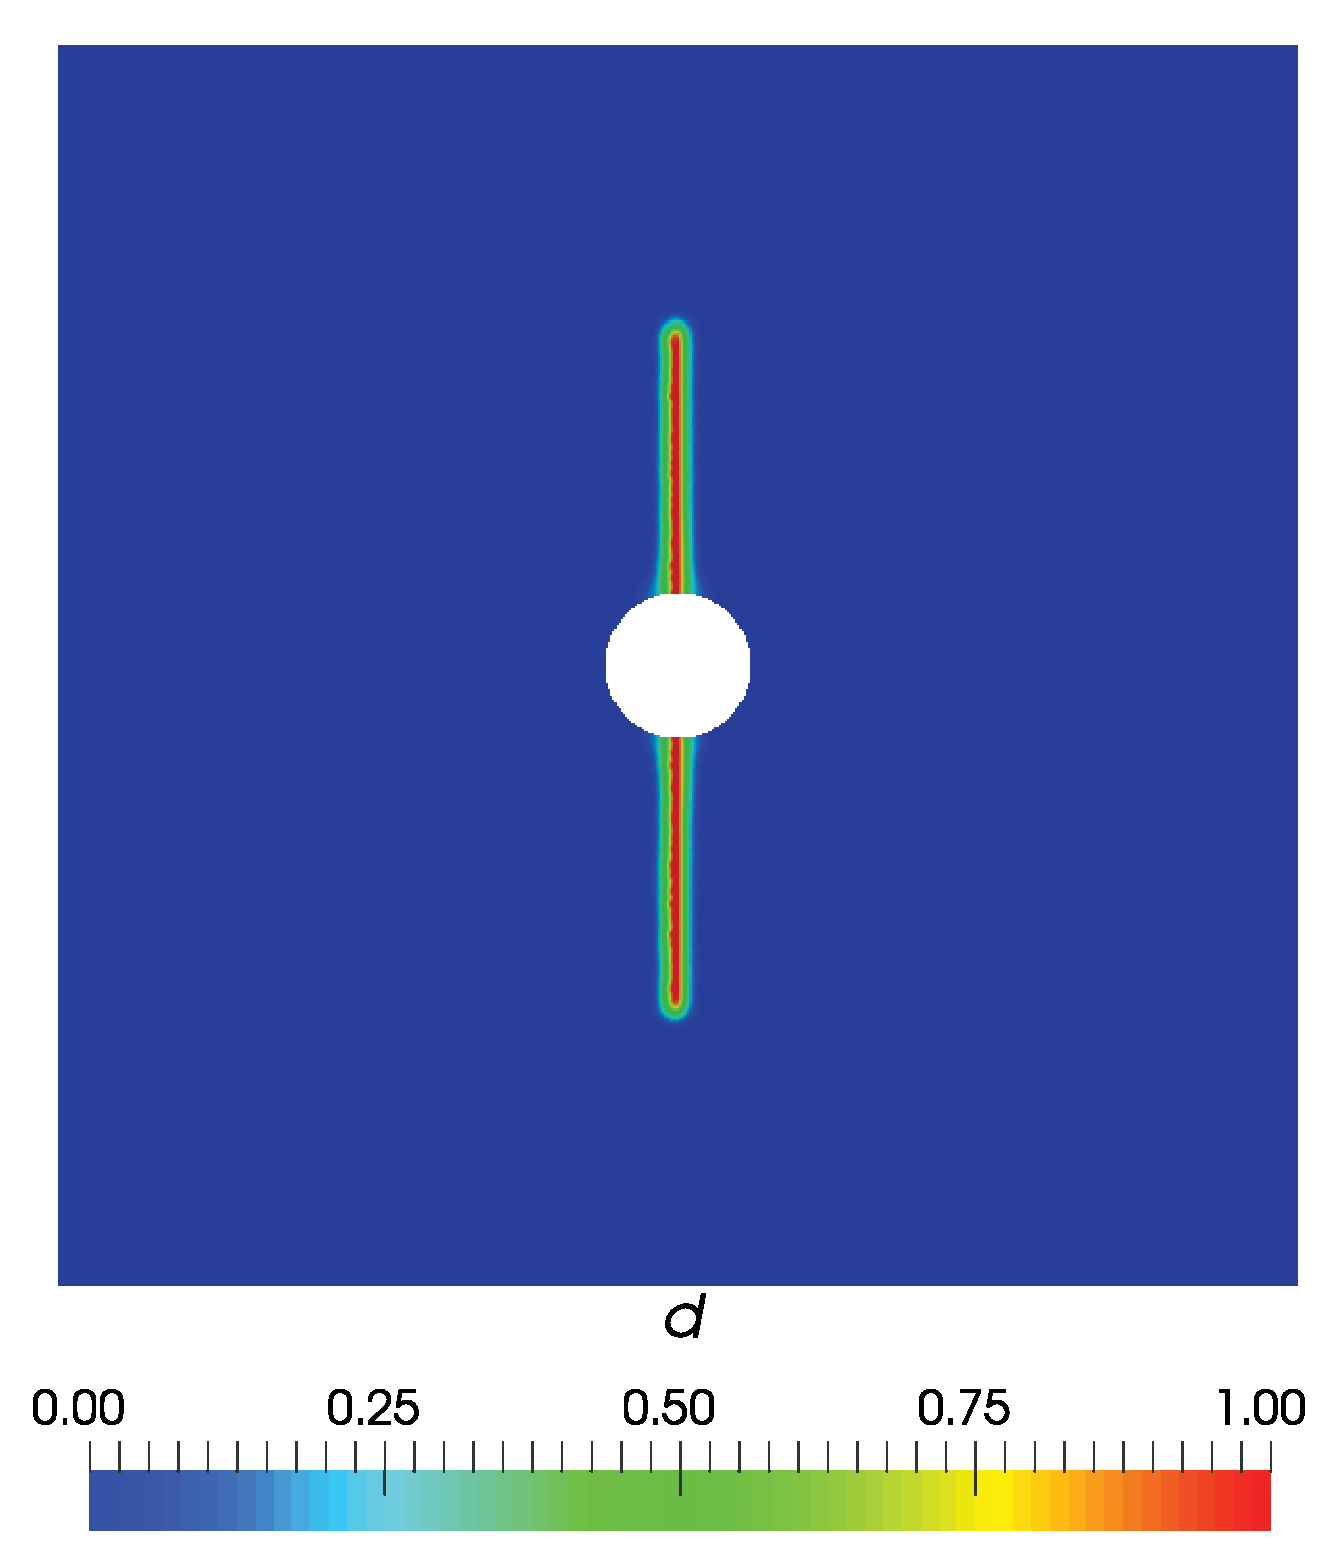
\includegraphics[width=60mm]{alpha_100.eps}\label{Fig:Gas_d_iii}}
%\subfloat[]{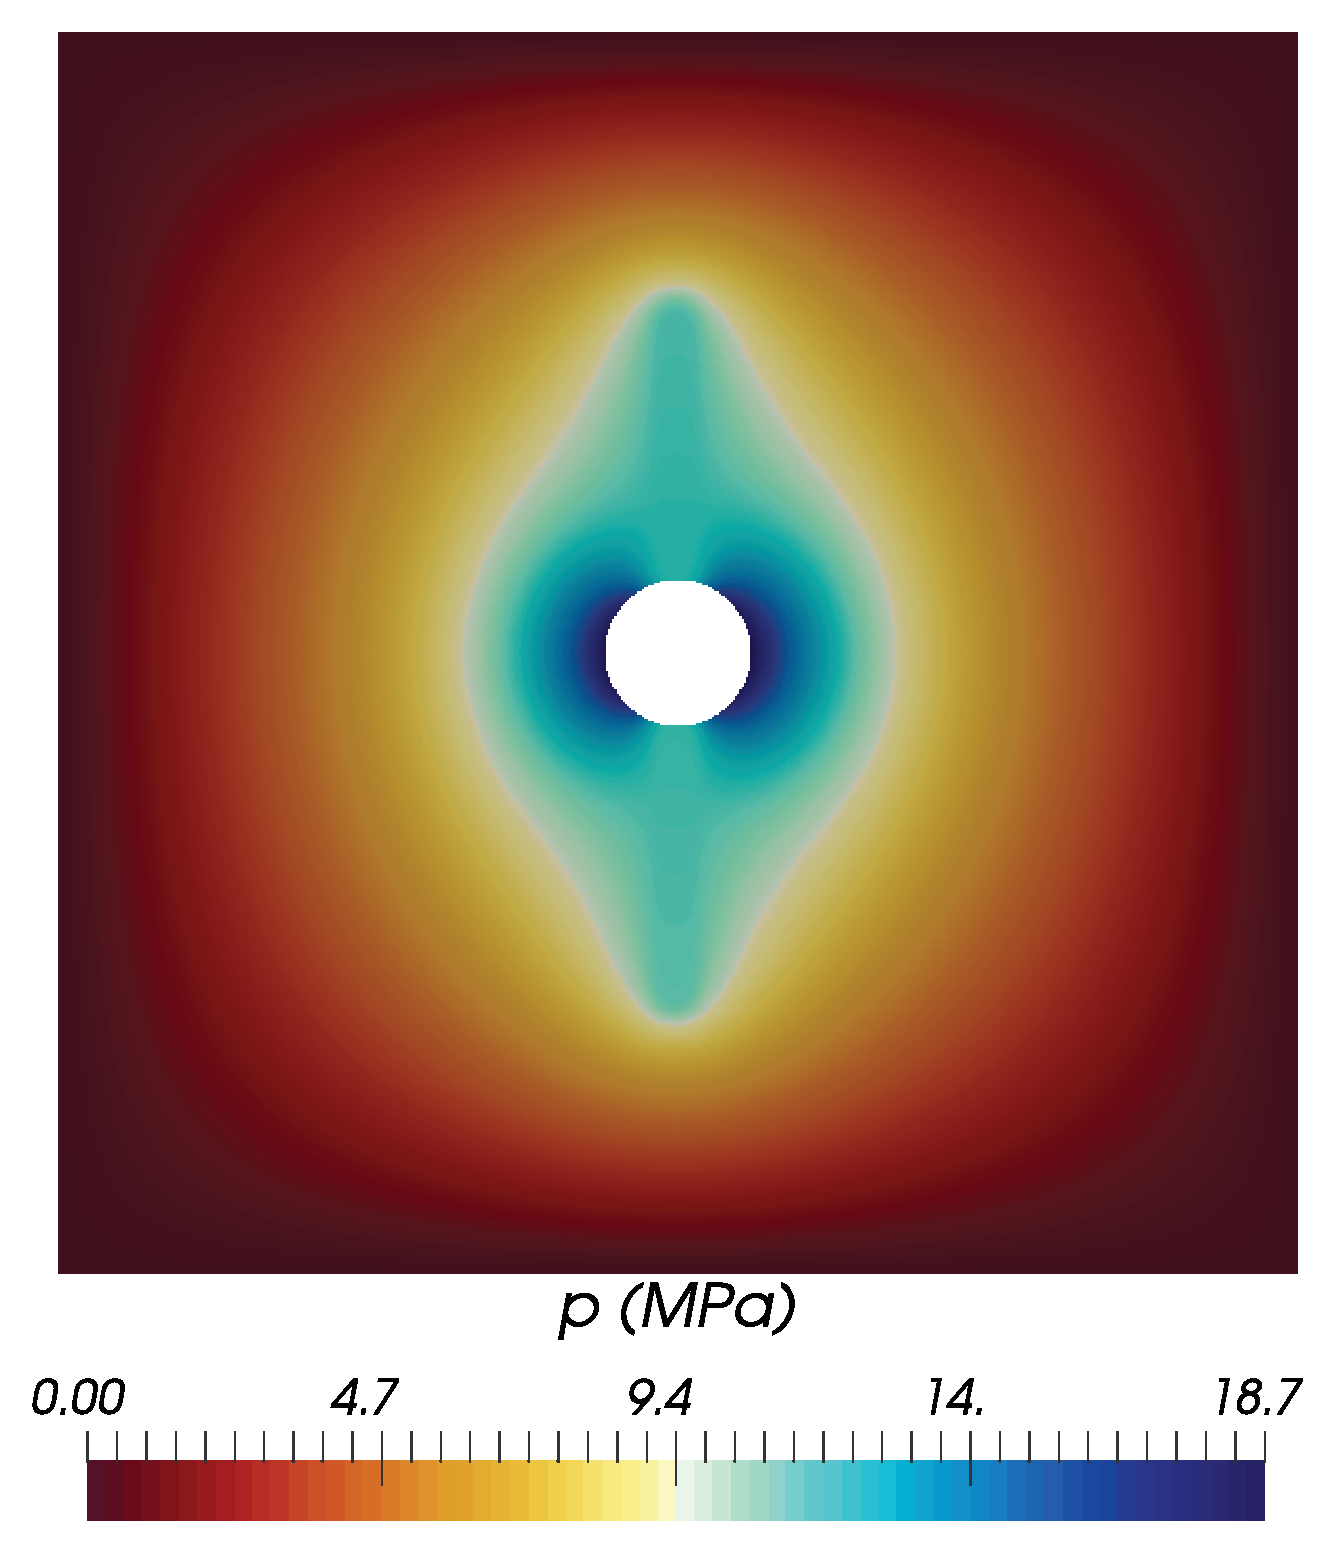
\includegraphics[width=60mm]{pressure_100.eps}\label{Fig:Gas_p_iii}}
%\caption{Left: Phase field diagram at different stages (\ref{Fig:Gas_d_i}) $t=0.5t_f$, (\ref{Fig:Gas_d_ii}) $t=0.75t_f$, and (\ref{Fig:Gas_d_iii}) $t=t_f$). Right: Pressure profile at (\ref{Fig:Gas_p_i}) $t=0.5t_f$, (\ref{Fig:Gas_p_ii}) $t=0.75t_f$, and (\ref{Fig:Gas_p_iii}) $t=t_f$.}
%\label{Fig:Gas_snapshots}
%\end{figure}




\begin{figure}[htbp]
\centering %
\subfloat[]{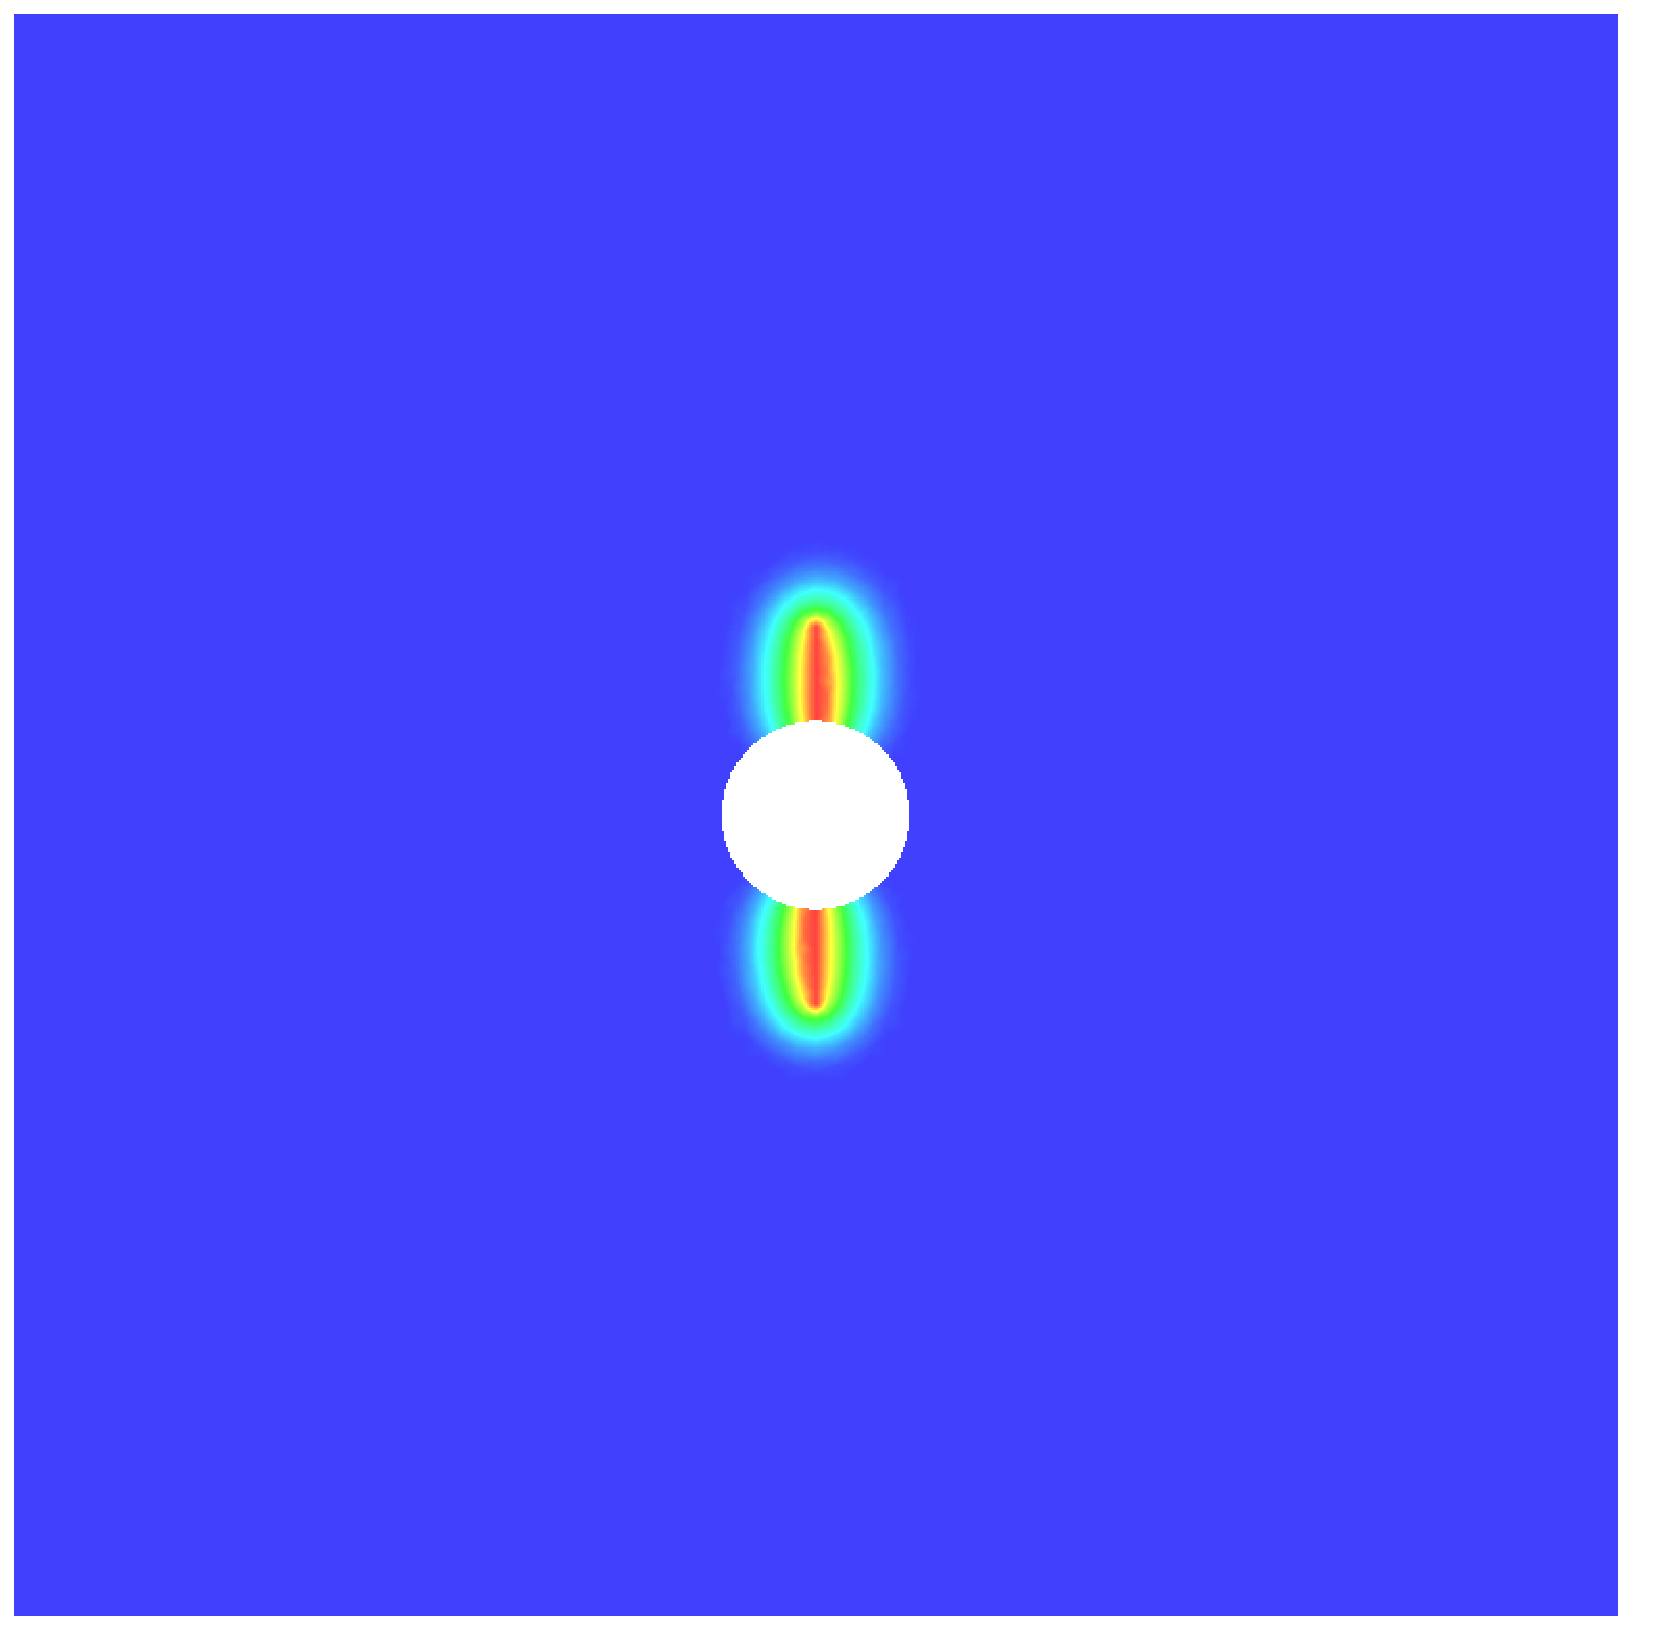
\includegraphics[width=60mm]{alpha25}\label{Fig:Gas_d_i}}
\subfloat[]{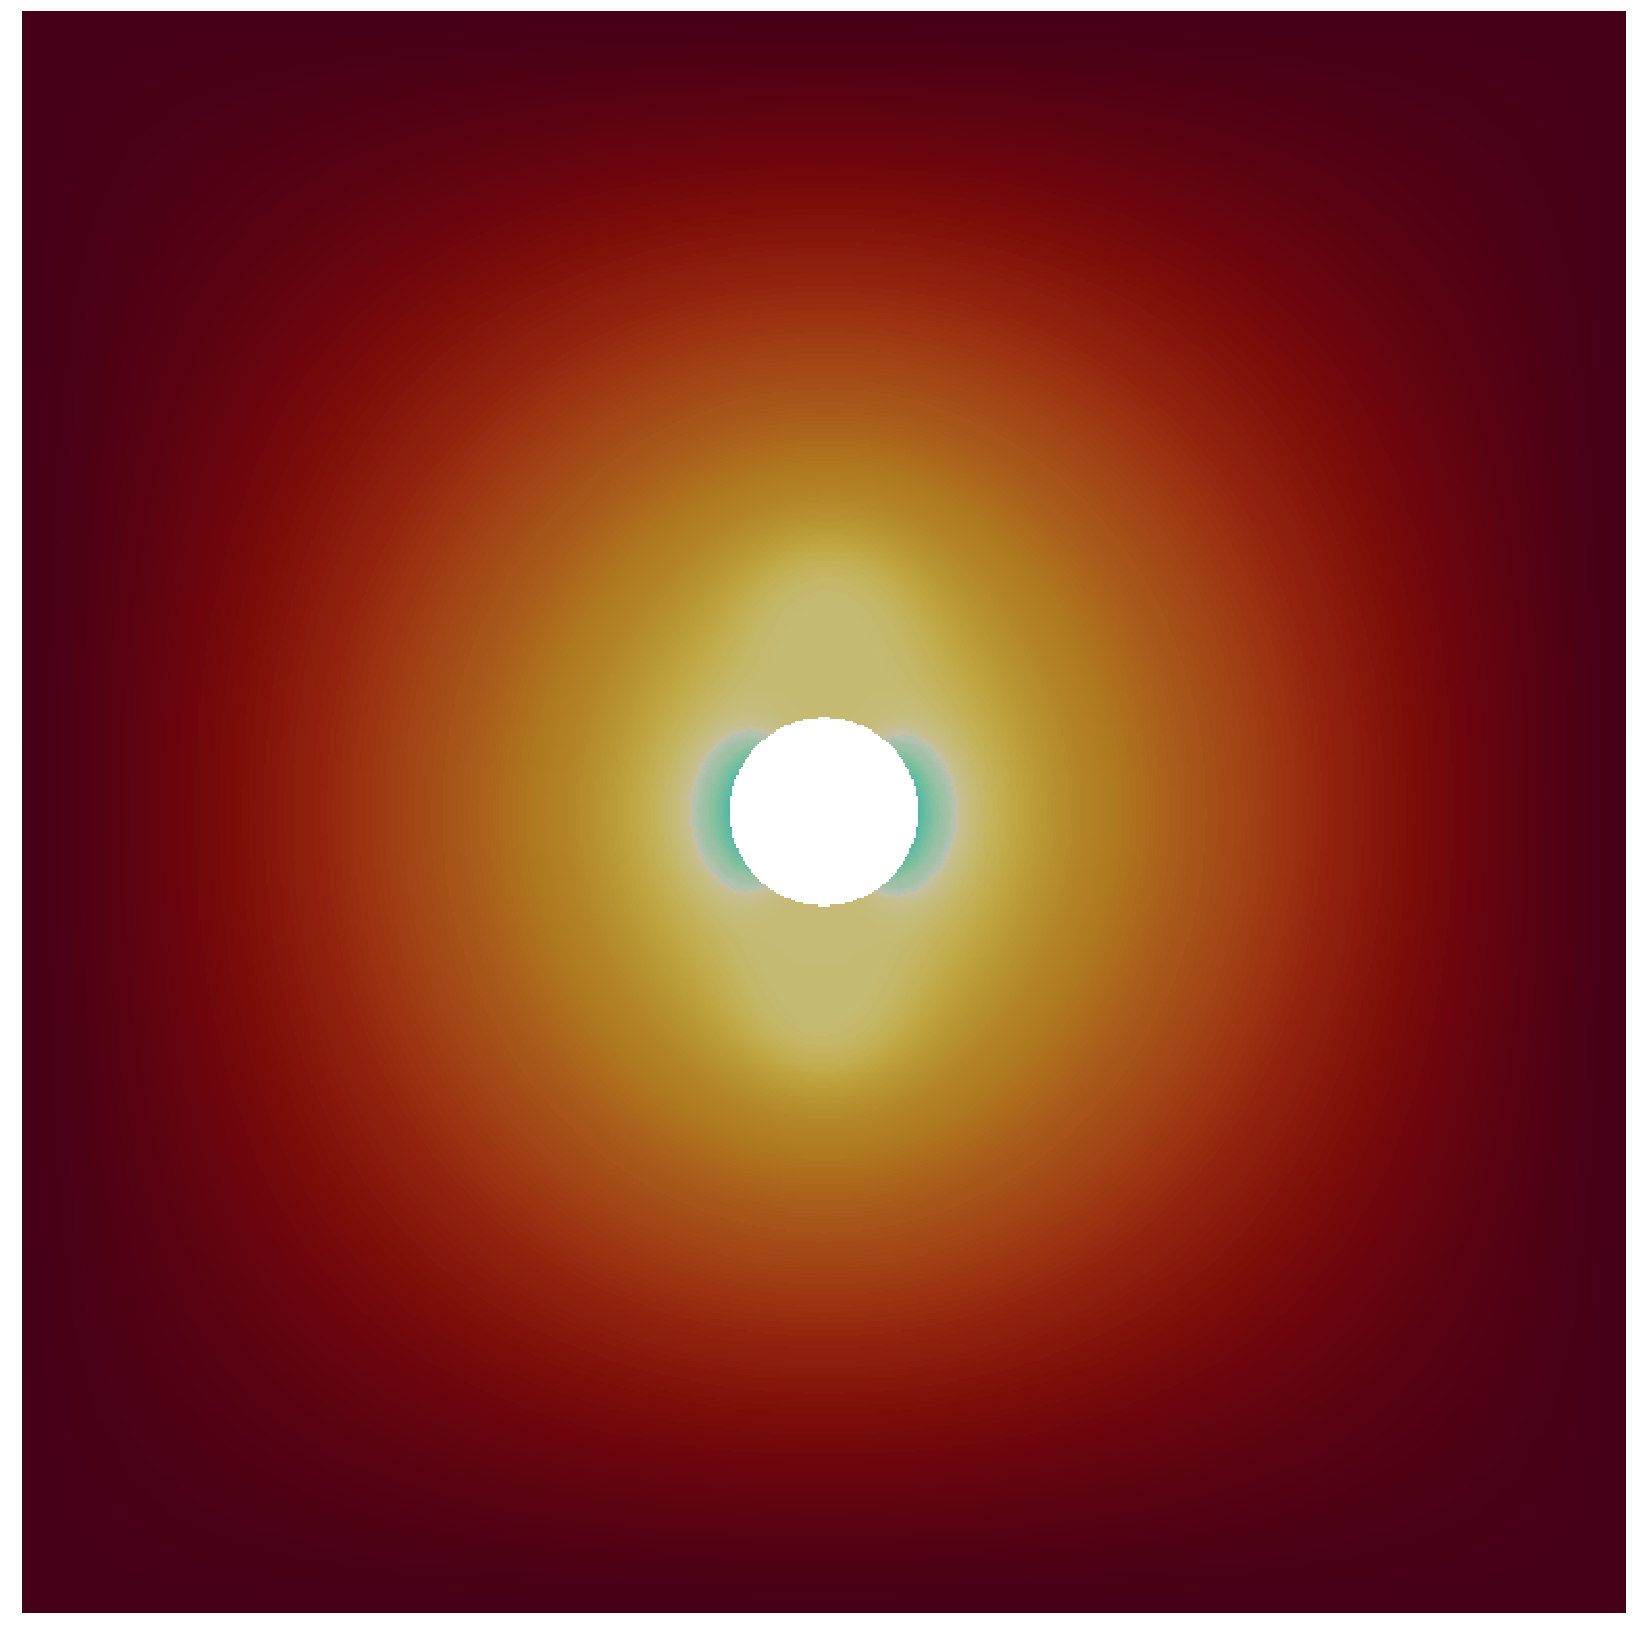
\includegraphics[width=60mm]{pressure25}\label{Fig:Gas_p_i}}\\
\subfloat[]{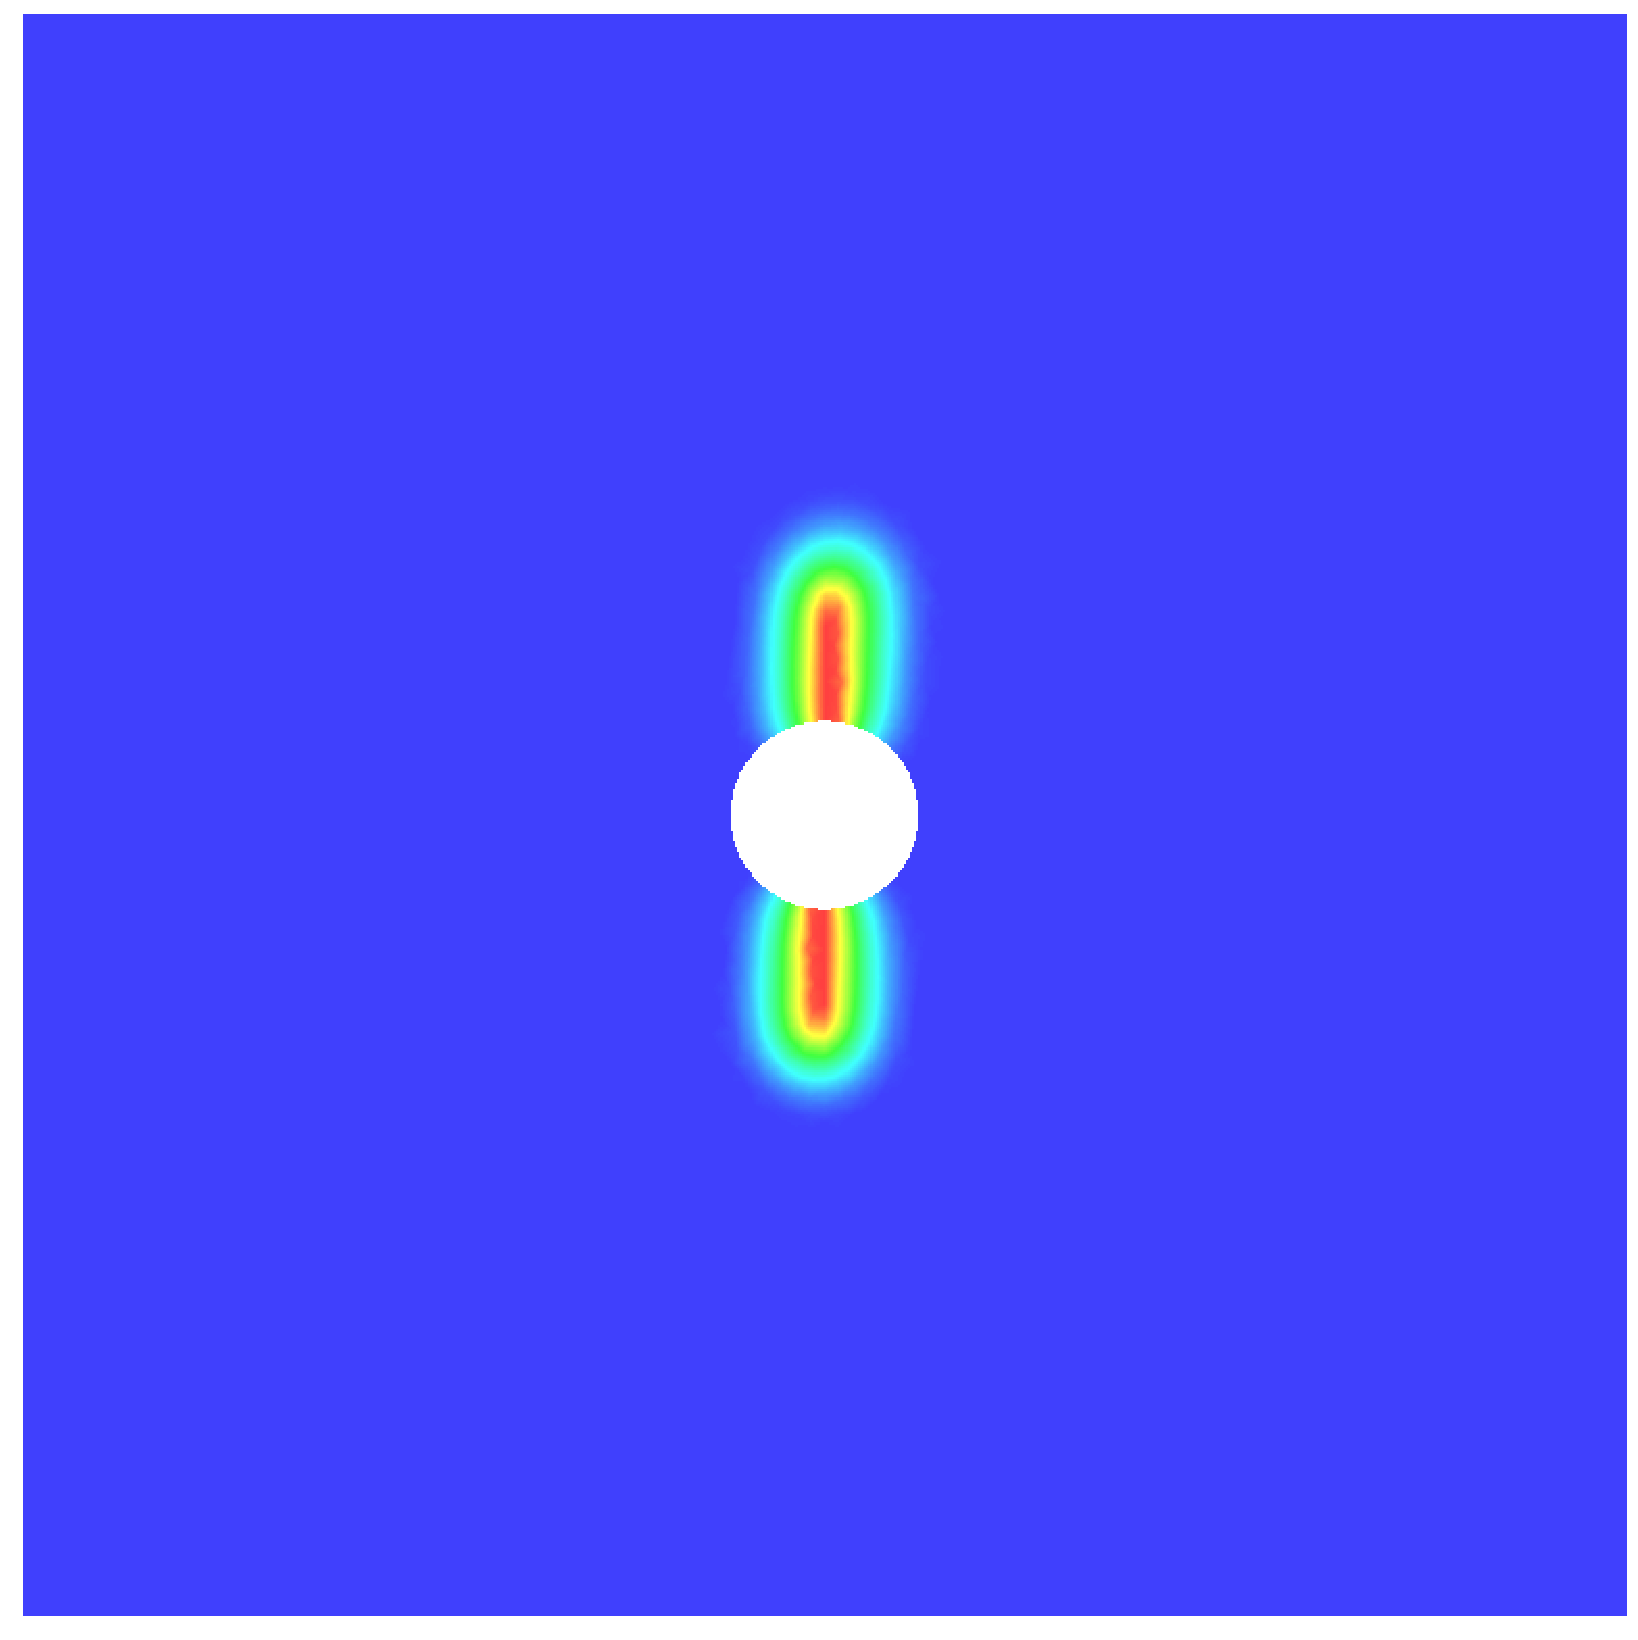
\includegraphics[width=60mm]{alpha37}\label{Fig:Gas_d_ii}}
\subfloat[]{
\includegraphics[width=60mm]{pressure37}\label{Fig:Gas_p_ii}}\\
\subfloat[]{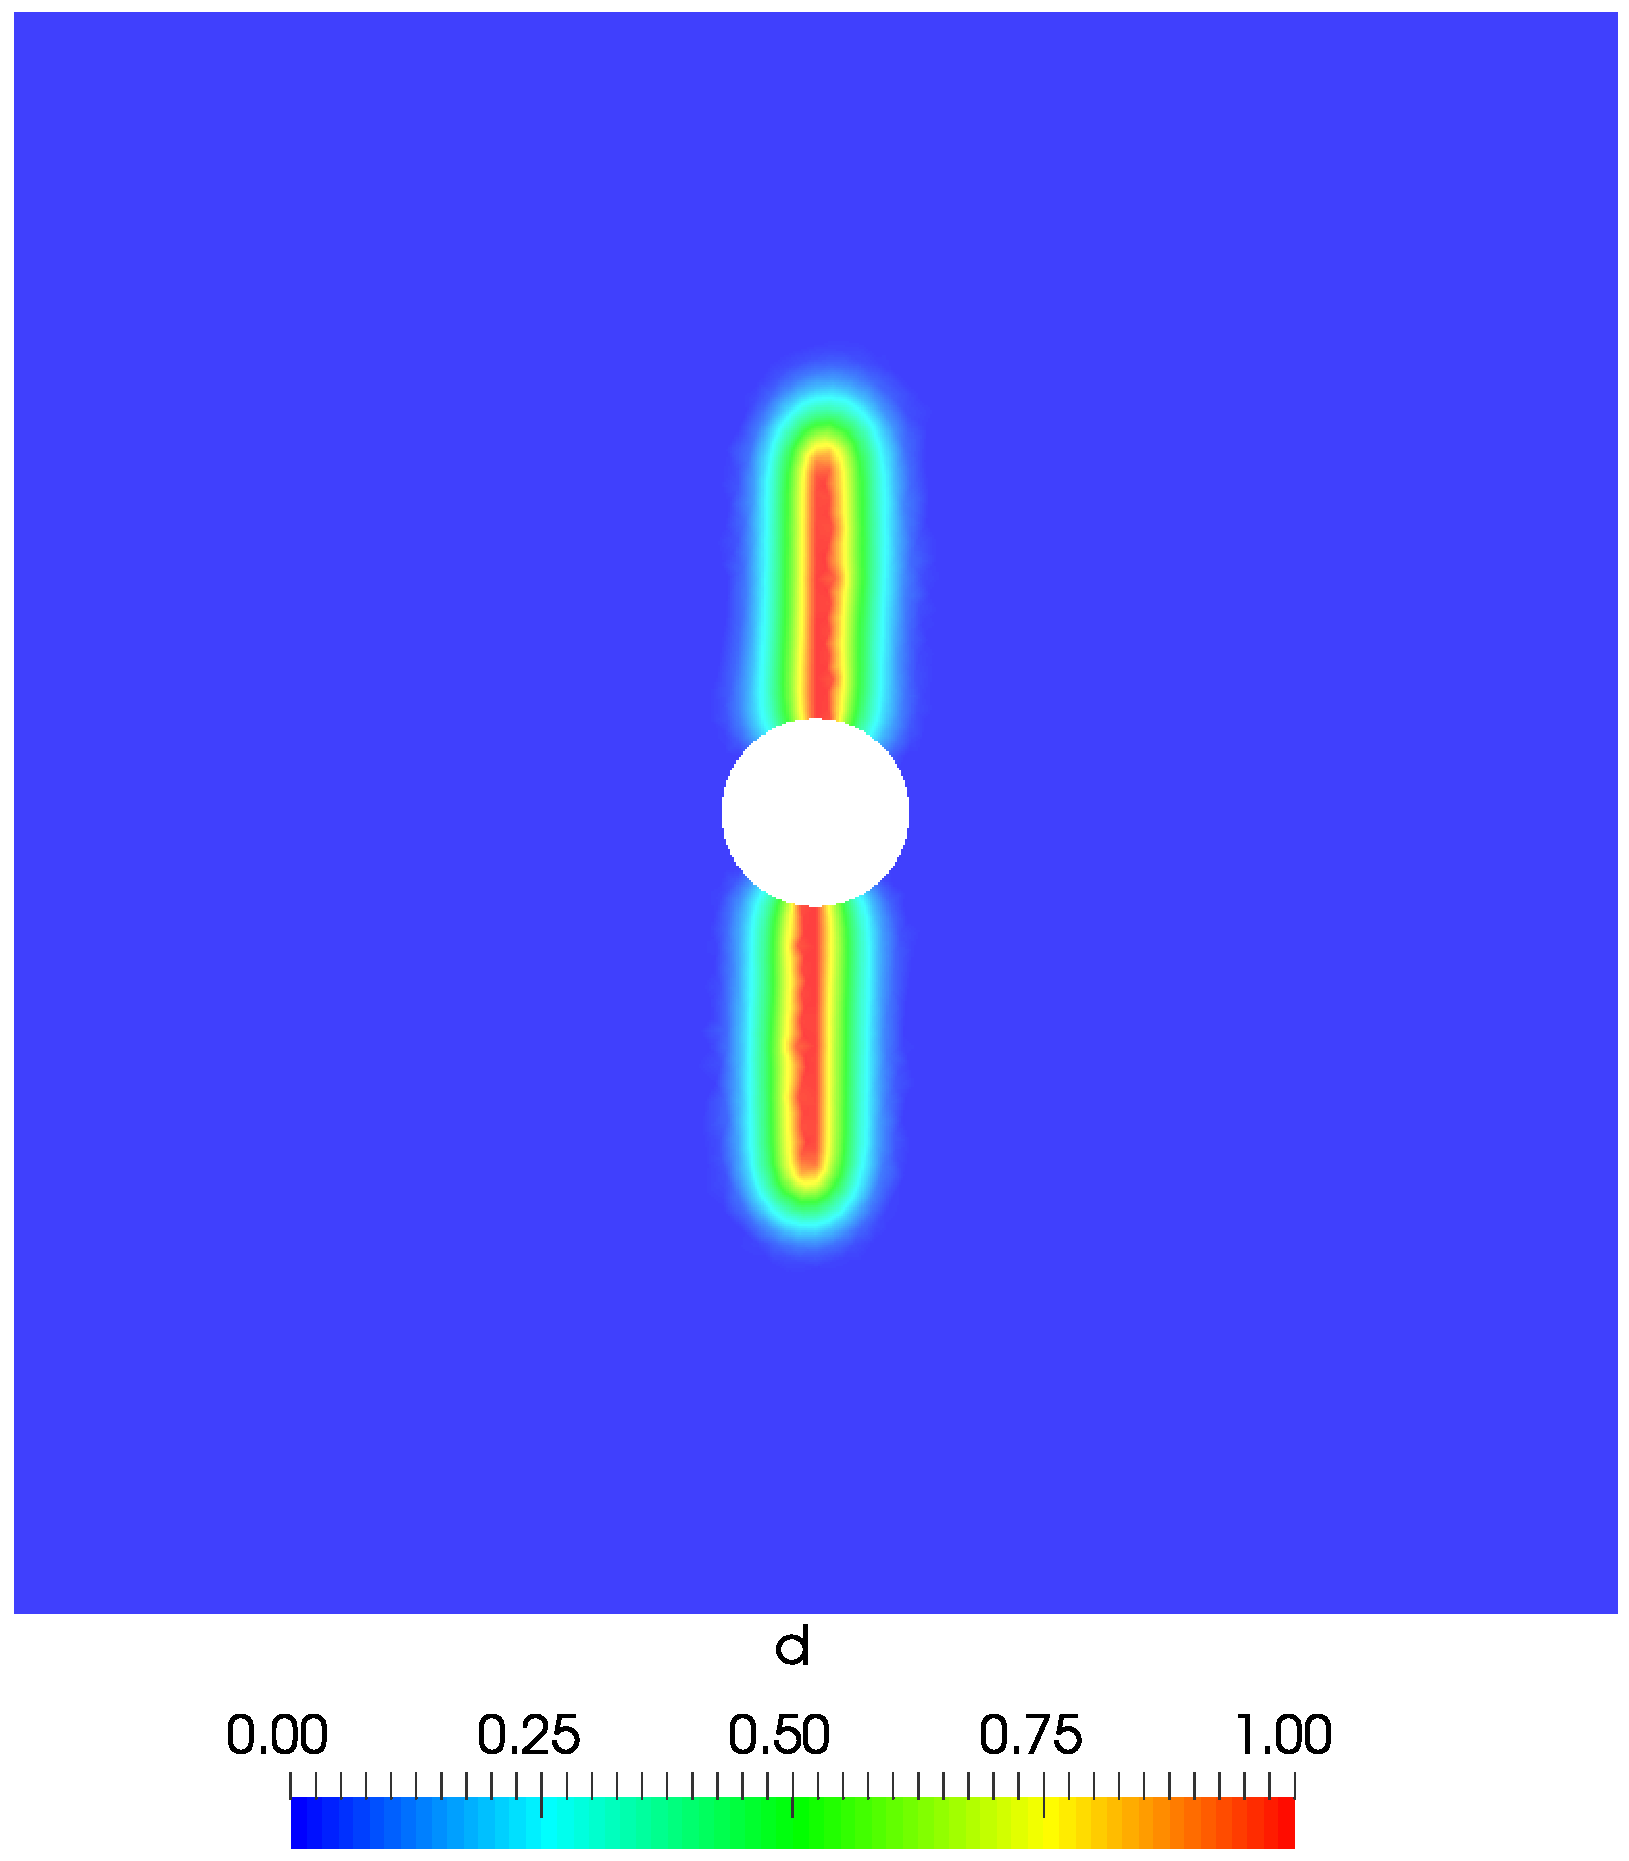
\includegraphics[width=60mm]{alpha49}\label{Fig:Gas_d_iii}}
\subfloat[]{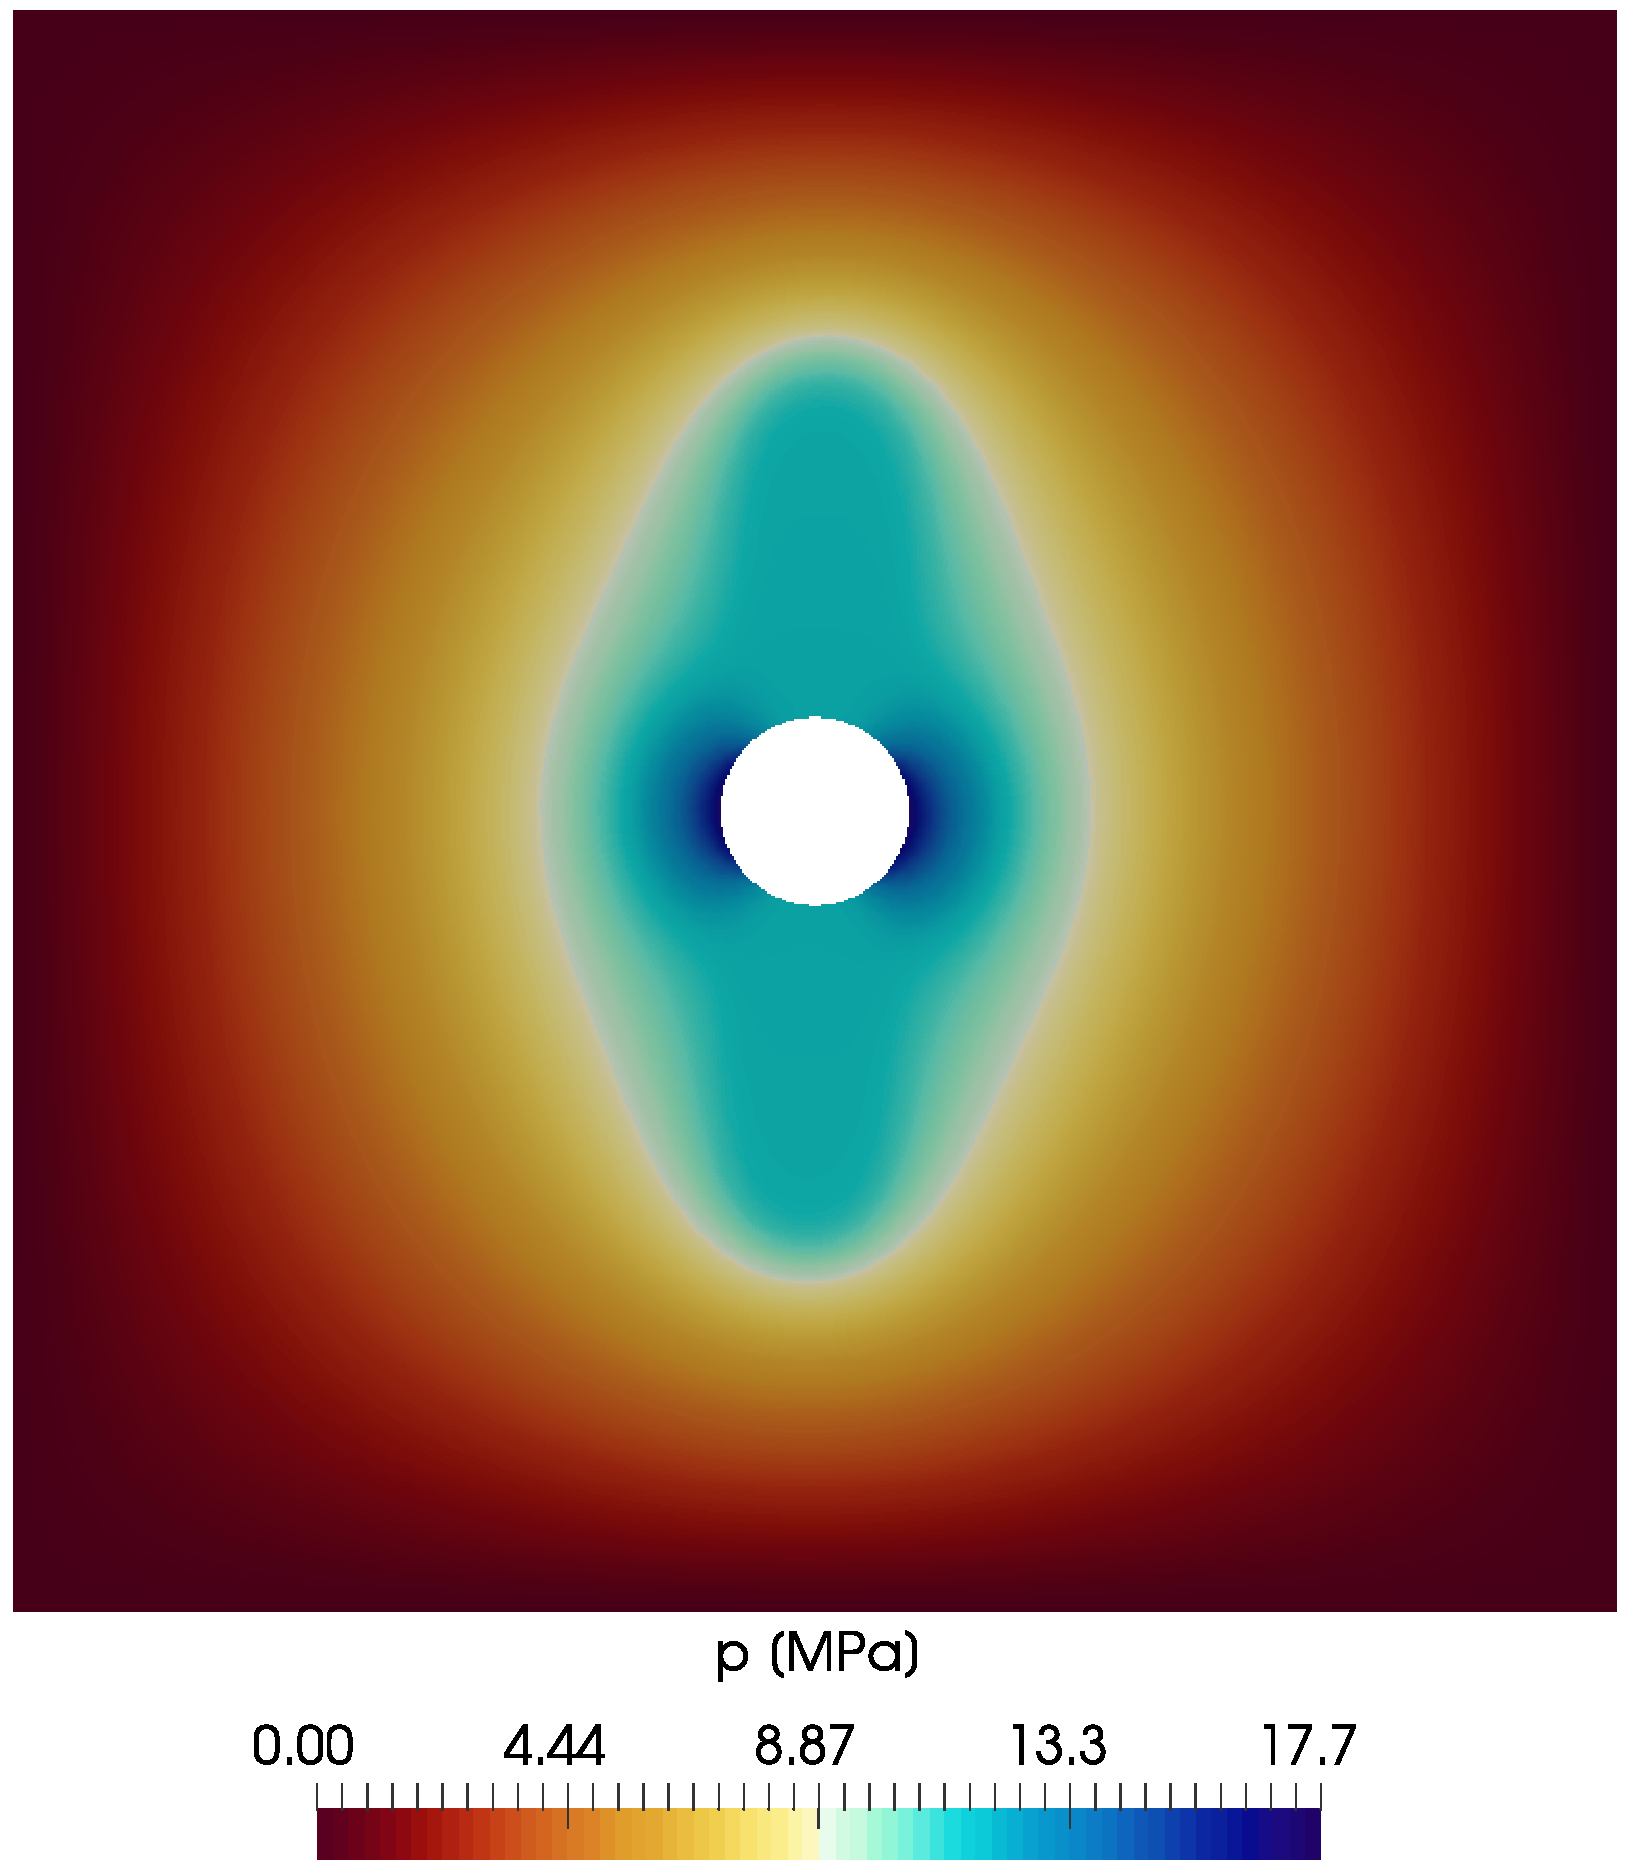
\includegraphics[width=60mm]{pressure49}\label{Fig:Gas_p_iii}}
\caption{Left: Phase field diagram at different stages (\ref{Fig:Gas_d_i}) $t=0.5t_f$, (\ref{Fig:Gas_d_ii}) $t=0.74t_f$, and (\ref{Fig:Gas_d_iii}) $t=t_f$). Right: Pressure profile at (\ref{Fig:Gas_p_i}) $t=0.5t_f$, (\ref{Fig:Gas_p_ii}) $t=0.74t_f$, and (\ref{Fig:Gas_p_iii}) $t=t_f$.}
\label{Fig:Gas_snapshots}
\end{figure}



%\todo[inline]{YS: The natural order is to first give OUR prediction of the breakdown pressure, then compare it with classical solutions.\\
%Vahid: The order is changed. See below.}

\begin{figure}
    \centering
    \includegraphics[width=0.6\textwidth]{Fracturelength_pressureboreholes_sigma_2}
    \caption{ The pressure at the top of the borehole (green line), and the fracture length function (blue line) as functions of time. The time when there is a sudden change of slope in $\mathcal{C}_{\ell}$ assumes the time corresponding to the breakdown pressure ($t=0.72t_f$) and the corresponding breakdown pressure is $p_b =10.9$ MPa. This is in agreement with H-F and H-W analytical solutions.}
	\label{Fig:Gas_pressure_Length_Sigma_i}
\end{figure}

Figure \ref{Fig:Gas_snapshots} shows the evolution of phase field diagram (left) and pressure profile (right) at different time steps. As seen, the fractures propagate along a straight line, and the pressure profile is accordingly distributed with the highest gradient around the borehole.

Next, we aim to calculate the breakdown pressure $p_b$, the pressure value when %at which the rapid drop in the injection pressure occurs and with 
the fractures start to propagate.
Figure \ref{Fig:Gas_pressure_Length_Sigma_i} illustrates the pressure evolution at the top of the borehole and the fracture length function. To estimate the breakdown pressure, first we output the fracture length with regard to \eqref{Eq:Gamma_ell}.  Then, we obtain the time when the slope suddenly changes in the fracture length function ($\mathcal{C}_{\ell}$), which is the time corresponding to the breakdown pressure (here $t\approx 0.72t_f$). Hence the breakdown pressure reads $p_b =10.9$ MPa. This value for $p_b$ is in agreement with H-F and H-W analytical solutions. Also, our results agree  with experiments results of Ishida \emph{et al.}~\cite{ishida2012acoustic} within 30\%, see Table \ref{Tab:preakdown_ISO_insitustress} and the next paragraph for more elaborations. 
%To validate our code we compare the numerical breakdown pressure with classical solutions$\cdots$
\begin{table}[htbp]
	\centering
	\caption{Breakdown pressure of numerical test and analytical solutions for $\sigma_1=\sigma_3=1$ MPa.}
	\begin{tabular}{l c c c c}
		\hline 
		& Numerical & H-F solution & H-W solution & Experimental \cite{ishida2012acoustic}  \\
		\hline 
		$p_b$ (MPa) & 10.9 & 11 &  9.1 & 8.44\\
		\hline      
	\end{tabular}
	\label{Tab:preakdown_ISO_insitustress}
\end{table}

\paragraph{Classical solutions of breakdown pressure} There exist two classical expressions to calculate the breakdown pressure. In the case without poroelastic effect the rock deformation does not penetrate into the pressurized fracture, the Hubbert-Willis (H-W) solution applies \cite{hubbert1972mechanics}:
\begin{equation*}
    p_b =3 \sigma_{3}- \sigma_{1}+\sigma_T,
\end{equation*}
in which the rock is assumed to be an elastic medium. When the porous medium is set, the Haimson-Fairhurst (H-F) solution is preferred \cite{haimson1967initiation}:
\begin{equation*}
    p_b=\dfrac{3\sigma_{3}- \sigma_{1}+\sigma_T+p_0}{1+\dfrac{\nu}{1-\nu}\alpha},
\end{equation*}
where we denote by $p_b$ the breakdown fluid pressure, $\sigma_{3}$, and $\sigma_{1}$ are the minimum and maximum principal stresses, respectively, and $\sigma_T$ is the rock's tensile strength.

\paragraph{Effect of $N$, $h$, and $\ell$ on the breakdown pressure}
Here we aim to study how the number of time steps $N$, the mesh size $h$, and the regularization length scale $\ell$ affect the value of breakdown pressure. As seen in Figure \ref{Fig:Gas_Pressure_parameters}, the plots show similar numerical results for the pressure evolution.

%\begin{figure}
%    \centering
%    \includegraphics[width=0.6\textwidth]{breakdownpressure_diff_ell_loadstep}
%        \caption{The pressure profile at the top of borehole for different {time steps, $N$}, and $\ell$.}
%    \label{Fig:Gas_Pressure_parameters}
%\end{figure}


\begin{figure}
    \centering
    \includegraphics[width=0.6\textwidth]{breakdownpressure_diff_ell_loadstep_2}
        \caption{Evolution of the pressure at the top of the borehole for different numbers of time steps $N$, mesh size $h$, and $\ell$.}
    \label{Fig:Gas_Pressure_parameters}
\end{figure}

%\todo[inline]{YS: Effect of the deviatoric part of the \emph{in situ} stress?\\Vahid: Changed.}
\paragraph{Breakdown pressure result of an anisotropic \emph{in situ} stress} In this example we set the maximum ($\sigma_1=3$ MPa) and minimum ($\sigma_3=2$ MPa)  \emph{in situ} stress. The other input data and boundary conditions are the same as aforementioned.

The pressure at the top of the borehole and the fracture length function, \eqref{Eq:Gamma_ell}, at different stages are  illustrated in Figure \ref{Fig:Gas_pressure_Length_Sigma_diff}. The breakdown time ($t\approx 0.77t_f$) and the corresponding breakdown pressure is $p_b =11.9$ MPa, see Table \ref{Tab:preakdown_anISO_insitustress}.

\begin{table}[htbp]
    \centering
    \caption{Breakdown pressure of numerical test and analytical solutions for $\sigma_1=3$ MPa and $\sigma_3=2$ MPa.}
    \begin{tabular}{l c c c}
    \hline 
           & Numerical & H-F solution & H-W solution \\
    \hline 
           $p_b$ (MPa)& 11.9 & 14 &  9.8 \\
    \hline      
    \end{tabular}
    \label{Tab:preakdown_anISO_insitustress}
\end{table}

\begin{figure}[htbp]
    \centering
    \includegraphics[width=0.6\textwidth]{Fracturelength_pressureboreholes_sigma_diff_2}
        \caption{The pressure at the top of the borehole (green line) and  the fracture length function (blue line) versus time for deviatoric \emph{in situ} stress are shown. The time ($t\approx 0.8t_f$) when there is a change of slope in the fracture length function ($\mathcal{C}_{\ell}$) should correspond to the breakdown pressure ($p_b=11.9$ MPa).}
    \label{Fig:Gas_pressure_Length_Sigma_diff}
\end{figure}

%\todo[inline]{Mostafa: Do we need keep this example? Since the results do not agree with experiments. Actually, the experiments indicate that the breakdown pressure is different for different fluids ($\mu$).\\Vahid: I added a few sentences to explain the case.}
\paragraph{Effect of dynamic viscosity on breakdown pressure} We conduct several numerical examples to investigate the effect of dynamic viscosity $\mu$ on the breakdown pressure $p_b$. 
In this set of examples an effective mesh size, the mesh size near the borehole or the fractures, $h\approx 1.6$ mm is adopted. Also, we set $\ell=2h$. In Figure \ref{Fig:Gas_Pressure_viscosity} we plot the pressure evolution up to the time when  $\mathcal{C}_\ell(t)$ changes slope, so that the end points correspond to the breakdown pressures. The results indicate that $p_b$ is approximately the same for different fluid viscosities, but the time when breakdown pressure reaches  is different. Figure \ref{Fig:Gas_Pressure_viscosity} demonstrates that the rock will break earlier for the fluid with bigger dynamic viscosity. Also it shows that regardless of the fracturing fluid, the breakdown pressure is slightly the same for all cases. This is in accordance with the physics that the breakdown pressure normally reflects the strength of the solid. However, Wang \emph{et al.}~\cite{wang2018influence} reported different breakdown pressures for different fluids which also agrees with some experiments \cite{ishida2012acoustic, ishida2016features}. We believe this discrepancy demands further research.

%\begin{figure}
%    \centering
%    \includegraphics[width=0.6\textwidth]{breakdown_diff_viscosity}
%         \caption{The pressure profile at the top of borehole for different $\mu$. As seen, even though $p_b$ is the same for different fracturing fluids, by increasing $\mu$, the breakdown pressure is reached in earlier time.}
%    \label{Fig:Gas_Pressure_viscosity}
%\end{figure}

%\todo[inline]{YS: Problems with Figure \ref{Fig:Gas_Pressure_viscosity}: $t_c$ should be $t_f$, and also the second legend shall be $\mu=1.00\times10^{-4}$ Pa$\cdot$s.\\
%Mostafa: It's edited}

\begin{figure}[htbp]
    \centering
    \includegraphics[width=0.6\textwidth]{breakdown_diff_viscosity_2}
         \caption{Evolution of the pressure at the top of the borehole for different $\mu$'s. As seen, even though $p_b$ is the same for different fracturing fluids, by increasing $\mu$, the breakdown pressure is reached earlier.}
    \label{Fig:Gas_Pressure_viscosity}
\end{figure}